\section{Distance between Energy Levels}
\label{sec:distance}
\subsection*{Current Wavelength Curve}
As mentioned in chapter \ref{sec:freeing} we already have transformed all data into the wavelength using the current wavelength curve. Because of that the order of the peaks has changed to 3 4 1 2. The next step is to transform the wavelength into the frequency using the formula $\nu=\frac{c}{\lambda}$, where $c$ is the speed of light in vacuum. The result can be seen in fig. \ref{image:fequency}.
\begin{center}
    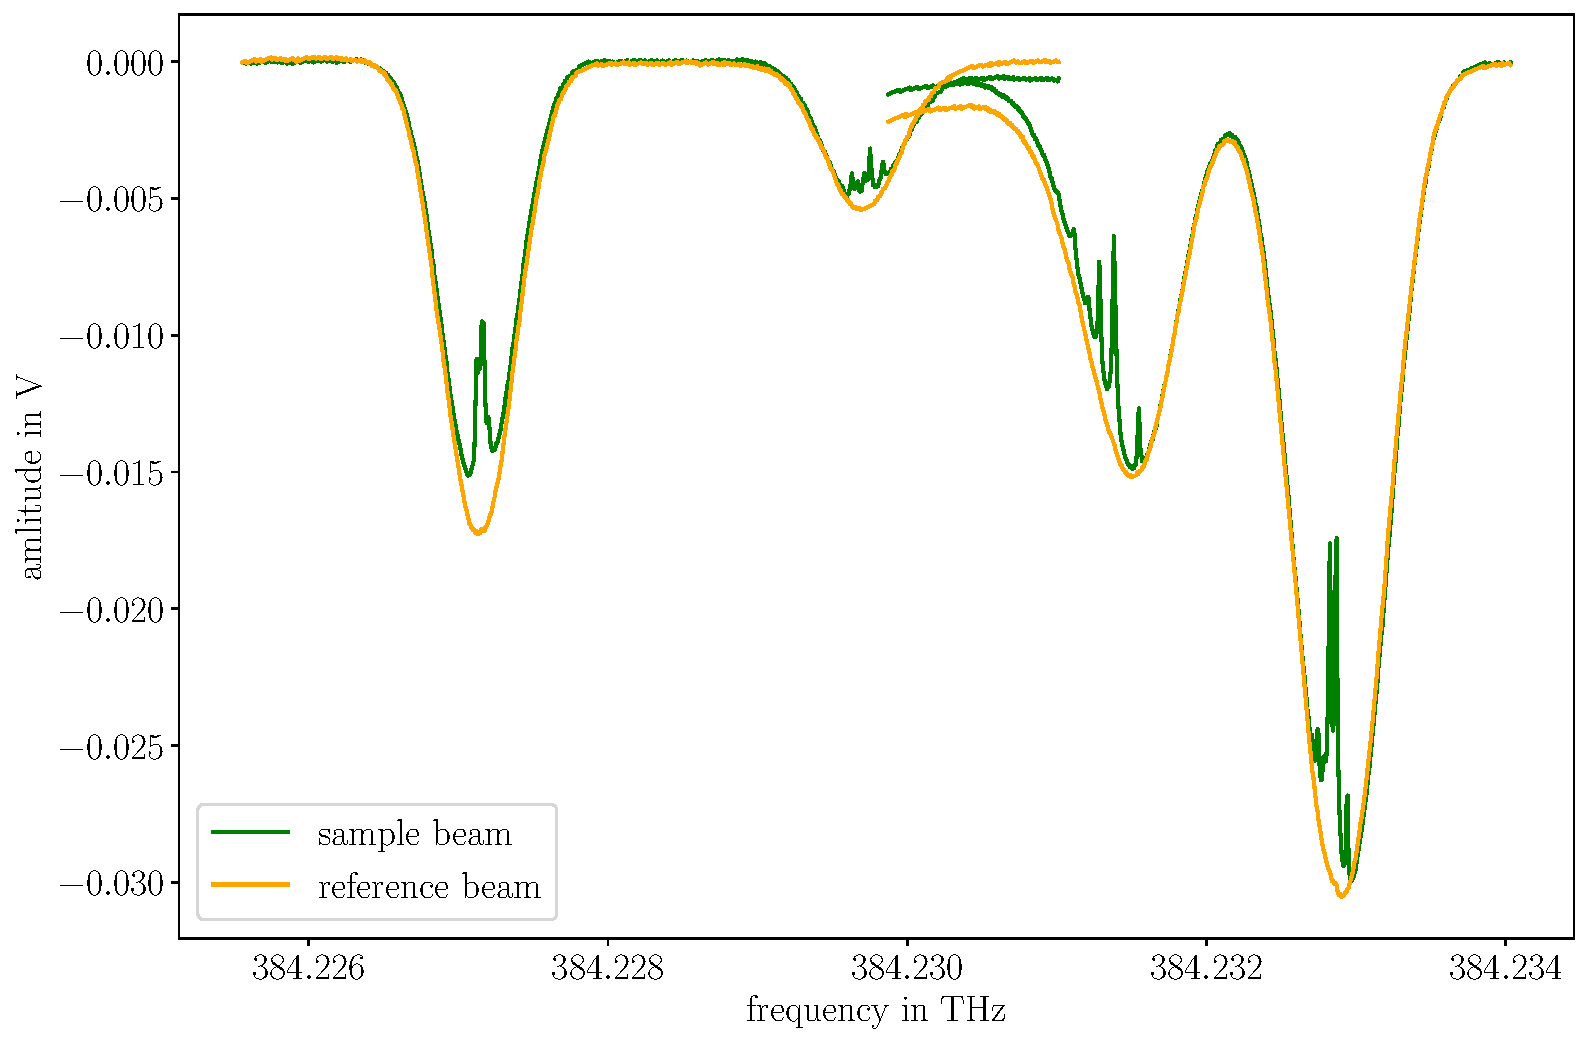
\includegraphics[scale=0.47]{Aufg-2/frequency_allPeak_Temp24.pdf}
    \captionof{figure}{Absorption spectrum after transformation to frequency}
    \label{image:fequency}
\end{center}
One can also see the occurrence of overlapping in fig. \ref{image:fequency} that is caused by the transformation from the laser current to the wavelength. It is possible to erase the overlapping lines from the data but for this evaluation it is necessary.
By using the same method as in chapter \ref{sec:freeing} to identify the peaks we obtain distance as followed:
\begin{center}
    \begin{tabular}{c | c}
        Peak area & $d_{current}$/THz\\
        \hline
        $2 \rightarrow 1$ & 0.00256\\
        $1 \rightarrow 4$ & 0.00181\\
        $4 \rightarrow 3$ & 0.00140\\
    \end{tabular}
    \captionof{table}{distances between the energy levels using current wavelength curve}
    \label{tab:currentMethode}
\end{center}
\subsection*{Fabry-Pérot Interferometer}
To calculate the distance of the energy level we start using the function of the Fabry-Pérot interferometer and insert the measured length $d$:
\begin{gather}
    \Delta\omega_{FSR} = \frac{c}{2nd} \overset{n=1}{=} \frac{c}{2d} \overset{d=\SI{1.515}{\metre}}{=} \SI{98.9}{\mega\hertz} 
\end{gather}
In the trendfree line of the interferometer we can count from 117.0455 mA to 137.6816 mA an amount of 97 maxima peaks what gives as relation:
\begin{gather}
    \frac{97\cdot \Delta\omega_{FSR}}{\SI{137.6816}{\milli\ampere}-\SI{117.0455}{\milli\ampere}} = 0.465\frac{\si{\giga\hertz}}{\si{\milli\ampere}}
\end{gather}
This means that 1 mA correspond to \SI{0.465}{\giga\hertz}. In following we use the table \ref{tab:identify} from chapter \ref{sec:freeing} for the information of the current for each peak and take the difference of them. That gives us in comparsion with the calculated data from table \ref{tab:currentMethode}:
\begin{center}
    \begin{tabular}{c | c c c}
        Peak area & difference/mA & $d_{interferometer}$/THz & $d_{current}$/THz\\
        \hline
        $1 \rightarrow 2$ & 5.5838 & 0.00260 & 0.00256\\
        $2 \rightarrow 3$ & 6.8314 & 0.00318 &   ---  \\
        $3 \rightarrow 4$ & 2.9248 & 0.00136 & 0.00140\\
    \end{tabular}
    \captionof{table}{distance between the energy levels using Fabry-Pérot interferometer and comparison to usage of current wavelength curve}
    \label{tab:interferometerMethode}
\end{center} 
In table \ref{tab:interferometerMethode} we can clearly see that both methods are equal in evaluation.
\newpage